\thesischapter{The Application of Real Time Maude to Model and Verify the European Rail Traffic Management System}
In the following we present the Maude \cite{MC03,Maude} and Real Time Maude \cite{PO02,PO04,RTMaude} tools and describe an approach using these tools to model and verify ERTMS \ref{}.


\section{The European Rail Traffic Management System}

\section{Formalising the European Rail Traffic Management System Using Hybrid Automata}
One formalism which we can use to real about systems such as ERTMS is hybrid automata \cite{TH96}.

\begin{mydef}[Hybrid Automaton]


\end{mydef}


\begin{figure} [h!]

\begin{center}
\begin{tikzpicture}[node distance = 3cm]


\node (A) [draw,regular polygon, regular polygon sides=5, minimum size=6 cm,outer sep=0pt] {};
\foreach \n in {1,...,5} {

    \pgfmathtruncatemacro{\value}{(\n - 1) * 50};
    \node at (A.corner \n) [anchor=360/5*(\n-1)+270] {D = \value};
    \node at (A.side \n) [anchor = 360/5 *(\n-1) +270] {$t_{\n}$};
}

\node (B) [draw, rectangle, rotate = 36] at (-1.9,2.6) {Train A};
\node (C) [draw, rectangle, rotate =72] at (3,-1) {Train B};

\end{tikzpicture} 
\end{center}

\label{fig:trackplan}
 \caption{Pentagon Example}
\end{figure}

\begin{comment}



\def\r{3} 
\def\sone{ \sin 32}
\def\stwo{\sin 72}
\def\cone{\cos 32}
\def\ctwo{\cos 72}
\coordinate(top) at (0,\r);
\coordinate(topleft) at ({ \r * -cos (36)},{ \r * -sin (36)});
\coordinate(topright) at ({ \r * cos (72)}, { \r * -sin (72)});
\coordinate(botleft) at ({ \r * - cos (36)},{ \r * sin (36)});
\coordinate(botright) at ({\r * sin (72)},{\r * cos (72)});

\tikzstyle{box1}=[circle, draw, text width = 2cm, font=\scriptsize]
\tikzstyle{box3}=[rectangle, draw, text width = 2cm, font=\scriptsize]
\tikzstyle{arrow}=[->, thick]
\tikzstyle{biarrow}=[<->,very thick,shorten >=7pt,shorten <=7pt]


\node (A) [font = \scriptsize]  at (topleft)                  {D =1500 };

\node (B) [font = \scriptsize]    at (botleft)          {D = 0};

\node (C)[font = \scriptsize] at (top)  { D = 1000
						};

\node (D)[font = \scriptsize] at (botright)  { D = 500
						};

\node (E) [font = \scriptsize] at (topright) {D = 2000};

\draw [arrow] (D) -- node[right] {$t_1$} (E);
\draw [arrow] (A) -- node[below = 10pt] {$t_4$} (B);
\draw [arrow] (B) --  node[above = 10pt] {$t_2$} (C);
\draw [arrow] (C) -- node [left] {$t_3$} (D);
\end{comment}
We have modelled the ETMS system controlling the pentagon example (see fig \ref{fig:trackplan}) using several hybrid automata. In this example the value $D(t)$ represents the distance from the start point at time $t$. 
It contains 2 trains $A$ and $B$ and 5 track circuits $l_0, \ldots , l_4$. The track is uni-directional allowing trains to travel from $0 - 2499$. 


\begin{figure} [h!]

\begin{center}
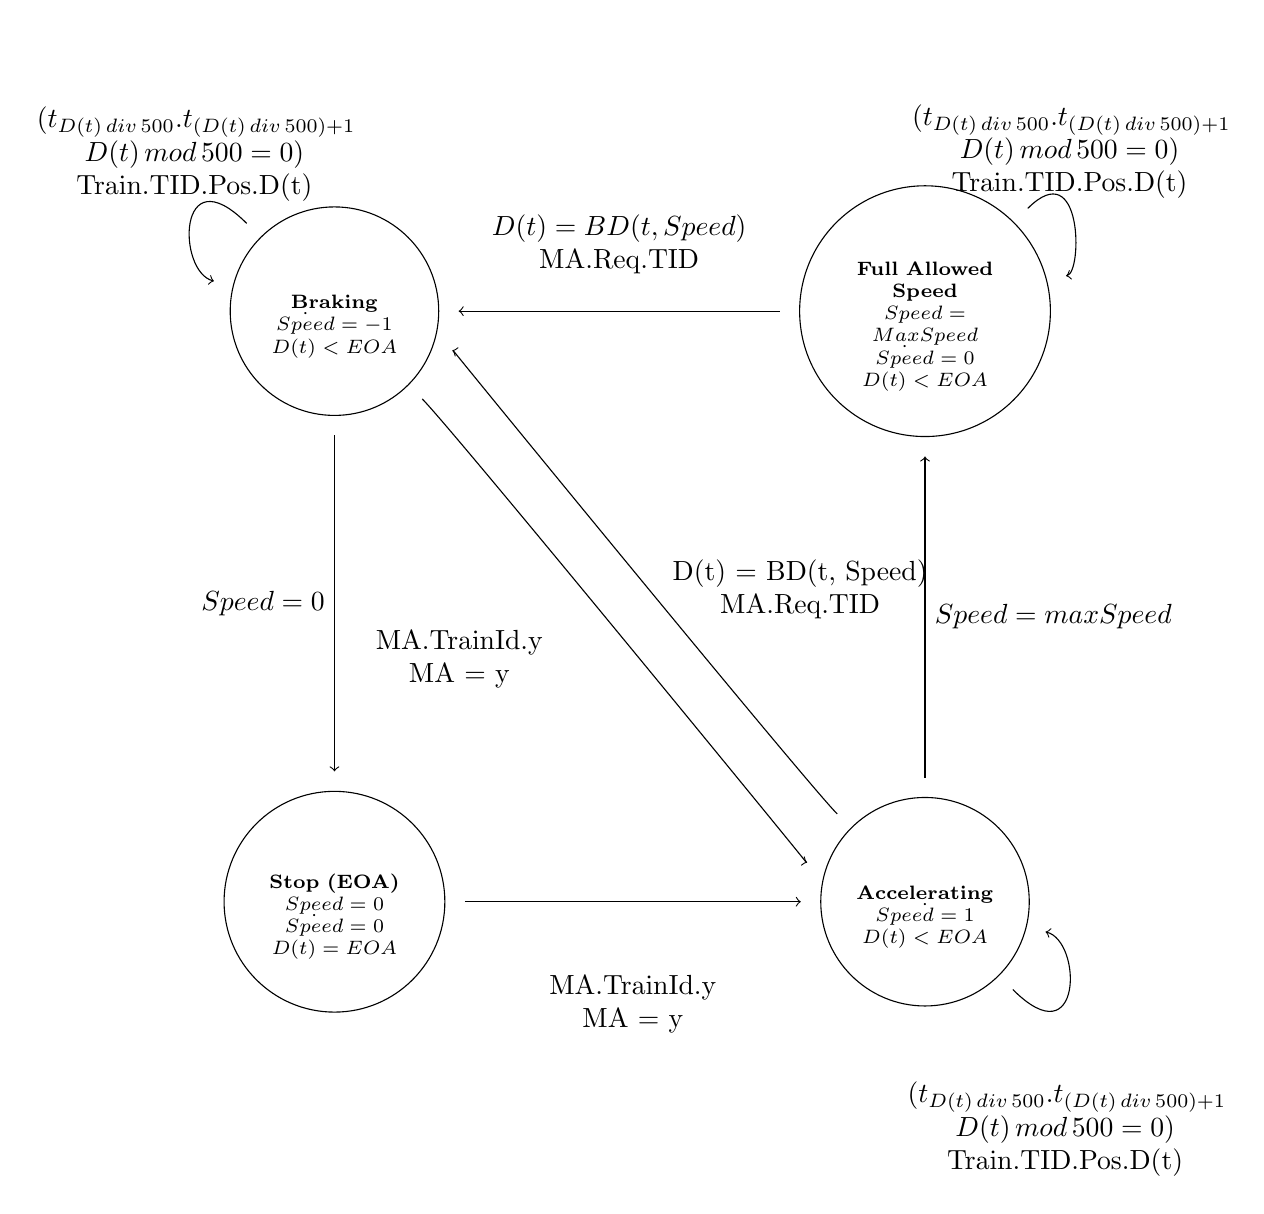
\begin{tikzpicture}[node distance = 2cm]

\tikzstyle{box1}=[circle, draw, text width = 2cm, font=\scriptsize]
\tikzstyle{box3}=[rectangle, draw, text width = 2cm, font=\scriptsize]
\tikzstyle{arrow}=[->,shorten >=7pt,shorten <= 7pt]
\tikzstyle{biarrow}=[<->,very thick,shorten >=7pt,shorten <=7pt]


\node (A) [box1]  at (0,0)                  {\begin{center} \textbf{Stop (EOA)} \\
							$Speed = 0$
                                                        $\dot{Speed} = 0$
							$D(t) = EOA$  \end{center}

                                            };

\node (B) [box1]    at (7.5,0)          {\begin{center} \textbf{Accelerating} \\
       $\dot{Speed = 1}$
       $D(t) < EOA$  \end{center}

};

\node (C)[box1] at (0, 7.5)  { \begin{center} \textbf{Braking}\\
					                   $\dot{Speed} = -1$ 
						           $D(t) < EOA$\end{center}
                                               
						};

\node (D)[box1] at (7.5, 7.5)  { \begin{center} \textbf{Full Allowed Speed }\\
					                   $Speed = MaxSpeed$
                                                            $\dot{Speed} = 0$
							    $D(t) < EOA$
                                                            \end{center}
                                               
						};


\draw [arrow] (B) -- node[right] {$Speed = max Speed$} (D);
\draw [arrow] (A) -- node[below = 10pt, text width = 4cm] {\begin{center}MA.TrainId.y\\ MA = y\end{center} } (B);
\draw [arrow] (D) --  node[above = 10pt,text width=4cm] {\begin{center}$D(t) = BD(t, Speed)$\\MA.Req.TID \end{center}} (C);
\draw [arrow] (C) -- node [left] {$Speed = 0$} (A);
\draw [arrow] (B)  .. controls +(-1.5cm,  1.5 cm) and +(1.5cm,  -0.5 cm ) .. node [right,text width=4cm] { \begin{center}D(t) = BD(t, Speed)\\MA.Req.TID \end{center}} (C);
\draw [arrow] (C) .. controls +(1.5cm,  -1.5cm) and +(-1.5cm, 0.5 cm ) ..   node [left,text width = 4cm] {\begin{center}MA.TrainId.y\\ MA = y\end{center} } (B);
\draw [arrow] (C) .. controls +(-2cm,  2cm) and +(-2cm, 0.5 cm ) ..   node [above = 5pt, text width = 4cm] {\begin{center}$(t_{D(t) \, div \, 500}.t_{(D(t) \, div \, 500) +1} $\\$D(t) \, mod \, 500 = 0)$\\Train.TID.Pos.D(t) \end{center}} (C);
\draw [arrow] (D) .. controls +(2cm,  2cm) and +(2cm, 0.5 cm ) ..   node [above = 5pt, text width = 4cm] {\begin{center}$(t_{D(t) \, div \, 500}.t_{(D(t) \, div \, 500) +1} $\\$D(t) \, mod \, 500 = 0)$\\Train.TID.Pos.D(t) \end{center}} (D);
\draw [arrow] (B) .. controls +(2cm,  -2cm) and +(2cm, -0.5 cm ) ..   node [below = 6pt, text width = 4cm] {\begin{center}$(t_{D(t) \, div \, 500}.t_{(D(t) \, div \, 500) +1} $\\$D(t) \, mod \, 500 = 0)$\\Train.TID.Pos.D(t) \end{center}} (B);

\end{tikzpicture} 
\end{center}

\label{fig:ContactOrders}
\end{figure}




\begin{mydef}[Interlocking Hybrid Automaton]
We define a hybrid automaton $H_{IL}$ as follows:
\begin{description}
\item[Variables] The state of the interlocking automaton consists of five boolean variables  $\underbrace{l_0, \ldots , l_4}_\text{Occupied/Free}$ and a variable $ReqID$ ranging over $\{0 , \ldots , 4 \}$.

\item[Control Graph] The control graph of the interlocking automaton consists of two control modes $\{Response, Idle \}$ with four control switches connecting them; $Response \to Idle$, $Idle \to Response$, $Response \to Response$, $Idle \to Idle$.

\item[Initial, invariant and flow conditions] \hspace*{0mm}
	\begin{itemize}
	\item $init(Idle) := [l_0 = Free, l_1 = Free, l_2 = Free, l_3 = Free, l_4 = Free]$.

	\end{itemize}

\item[Jump Conditions] \hspace*{0mm}

	\begin{itemize}
	\item $jump(Idle \to Response) :=  Req.z , ReqId' = z$

	
	\item $jump(Response \to Idle) := if \ (l_{ReqId} = Free \wedge l_{ReqId +1 \, mod \, 5} = Free) \ then \ Grant. ReqId \ else \ Deny.ReqId$ 

	\item $jump(Idle \to Idle) := l_x. l_{x+1} , [l_x' = Free, l_{x+1}' = Occupied]$

	\item $jump(Response \to Response) := l_x. l_{x+1} , [l_x' = Free, l_{x+1}' = Occupied]$


	\end{itemize}

\item[Events] \hspace*{0mm}
\begin{itemize}
	\item $event (Idle \to Response) := Req.z$
	\item $event(Response \to Idle) :={Grant.z,Deny.z}$
	\item $event(Idle \to Idle) := l_x.l_{x+1}$
	\item $event(Response \to Response) := l_x.l_{x+1}$	
\end{itemize}

\end{description}
\end{mydef}

Secondly we define a hybrid automaton $H_{T}$ which models an individual train. 

\begin{mydef}[Train Automaton]

We define a hybrid automaton $H_{T}$ as follows:
\begin{description}
\item[Variables] The state of the interlocking automaton consists of $\underbrace{D(t), EoA}_\text{0, \ldots , 2499}$, \newline $\underbrace{Speed, \dot{Speed}, MaxSpeed, TID}_{\mathbb{N}}$.

\item[Control Graph] The control graph of the interlocking automaton consists of four control modes $\{Stop (EoA), \, Braking, \, Accelerating, \, Full \, Allowed \, Speed \}$.

\item[Initial, invariant and flow conditions] \hspace*{0mm}
	\begin{itemize}
	\item $init(Stopped) :=   D(t) < EoA  $.

	\item $inv(Full Allowed Speed) :=   \dot{Speed} = 0 \wedge D(t) < EoA$ 

	\item $inv(Accelerating) := D(t) < EoA$

	\item $inv(Braking)  := D(t) < EoA$
	
	\item $inv(Stop (EoA)) := Speed = 0$ 

	\item $flow(Accelerating):= \dot{Speed} = 1$ 
	
	\item $flow(Braking) := \dot{Speed} = -1$
	
	\end{itemize}

\item[Jump Conditions] \hspace*{0mm}

	\begin{itemize}
	\item $jump(Full Allowed Speed \to Full Allowed Speed) := l_{D(t) \, div \, 500}.l_{(D(t) \, div \, 500) +1} \wedge D(t) \, mod \, 500 = 0$
\item $jump(Braking \to Braking) = l_{D(t) \, div \, 500}.l_{(D(t) \, div \, 500) +1} \wedge D(t) \, mod \, 500 = 0$
\item $jump(Accelerating \to Accelerating) = l_{D(t) \, div \, 500}.l_{(D(t) \, div \, 500) +1} \wedge D(t) \, mod \, 500 = 0$

	\item $jump(Stop (EoA) \to Accelerating) := MA.TID.y \wedge EoA' = y$ 
	
	\item $jump(Braking \to Accelerating) := MA.TID.y \wedge EoA' = y$ 

	\item $jump(Accelerating \to Braking) := D(t) = BD(t, Speed) \wedge MA.Req.TID$

	\item $jump(Full Allowed Speed \to Braking) := D(t) = BD(t, Speed) \wedge MA.Req.TID$

	\item $jump(Accelerating \to Full Allowed Speed)$ := Speed = MaxSpeed
	
	\item $jump(Braking \to Stop (EoA)) := Speed = 0$

	\end{itemize}

\item[Events] \hspace*{0mm}
\begin{itemize}
	\item $event (Stop (EoA) \to Accelerating) := MA.TID.y$
	\item $event (Braking \to Accelerating) := MA.TID.y$
	\item $event(Full Allowed Speed \to Full Allowed Speed) := l_{D(t) \, div \, 500}.l_{(D(t) \, div \, 500) +1} \wedge D(t) \, mod \, 500 = 0$
\item $event(Braking \to Braking) = l_{D(t) \, div \, 500}.l_{(D(t) \, div \, 500) +1} \wedge D(t) \, mod \, 500 = 0$
\item $event(Accelerating \to Accelerating) = l_{D(t) \, div \, 500}.l_{(D(t) \, div \, 500) +1} \wedge D(t) \, mod \, 500 = 0$

	\item $event(Accelerating \to Braking) = MA.Req.TID$
	\item $event(Full Allowed Speed \to Braking) = MA.Req.TID$
\end{itemize}

\end{description}
\end{mydef}

In both $H_{IL}$ and $H_T$ we make use of an event $l_x.l_{x+1}$ to capture the movement of the train from one track segment to the next. In the above hybrid automaton modelling the trains we make use of a function $BD$ that calculates location required to stop at the EOA based on the trains speed. The point at which the train should break would then be modelled as $BD(EOA, speed) = EOA - \frac{speed ^2}{2}$ mod 2500.



This hybrid automaton has $4$ control modes namely Braking (Auth), Full Allowed Speed, Accelerating and Stopped and has $5$ variables namely $Maxspeed$,$D(t)$ (Position),  $Speed$, $\dot{Speed}$ and $EoA$. We have that $D(t) \leq EOA$ is an invariant of the stopped mode and $D(t) \leq EOA$ is an invariant of all other control modes.
We define a transition with the event $l_x.l_{x+1}$ which is triggered by the condition $D \,  mod \, 500 = 0$ in the modes $Full Speed$, $Accelerating$ and $Brake$ and causes TC = x +1. 
The simplest way to model deceleration would be to assume that the trains speed decreases at $-1$ unit of distance per unit of time.   We compose both the automata for both the interlocking and the hybrid $H_{IL} || H_{T}$. It is possible for a new MA $EOA'$ with $EOA < EOA'$ to be received in the $Braking$ and $Stopped$ states. 



\begin{figure} [h!]

\begin{center}
\begin{tikzpicture}[scale = 0.60]

\tikzstyle{box1}=[circle, draw, text width =3cm]
\tikzstyle{box3}=[rectangle, draw, text width = 2cm, font=\scriptsize]
\tikzstyle{arrow}=[->,shorten >=7pt,shorten <= 7pt]
\tikzstyle{biarrow}=[<->,very thick,shorten >=7pt,shorten <=7pt]



\node (B) [box1]    at (7.5,0)          {\begin{center} \textbf{Idle} \\ \end{center}

};

\node (C)[box1] at (0, 7.5)  { \begin{center} \textbf{Response}\\ \end{center}                                               
						};


\draw [arrow] (B)  .. controls +(-1.5 cm,  2.75 cm) and +(4.5cm,  -2.5cm ) .. node [right = 2cm, above = 0.5cm, text width=4cm] {Req.z} (C);
\draw [arrow] (C) .. controls +(1cm,  -3cm) and +(-2.75cm, 1 cm ) ..   node [left = 3 cm, below, text width = 6cm] {$Grant.z \  t_{z} = free \wedge t_{z + 1 \, mod \, 5} = free$\\$Deny.z \ Otherwise$} (B);


\end{tikzpicture} 
\end{center}

\label{fig:ILAuton}
\end{figure}


\begin{comment}

\begin{figure} [h!]

\begin{center}
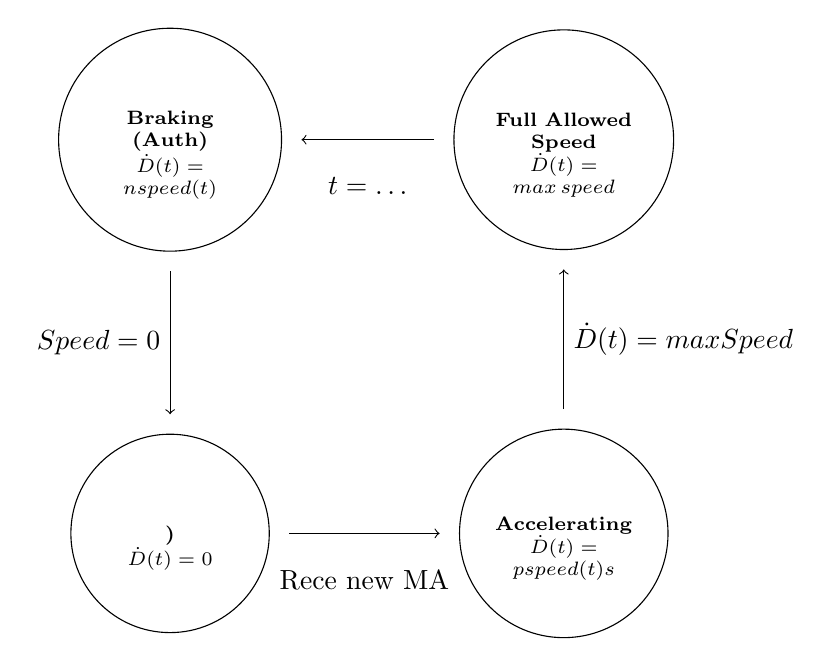
\begin{tikzpicture}[node distance = 3cm]

\tikzstyle{box1}=[circle, draw, text width = 2cm, font=\scriptsize]
\tikzstyle{box3}=[rectangle, draw, text width = 2cm, font=\scriptsize]
\tikzstyle{arrow}=[->,shorten >=7pt,shorten <=7pt]
\tikzstyle{biarrow}=[<->,very thick,shorten >=7pt,shorten <=7pt]


\node (A) [box1]  at (0,0)                  {\begin{center} \textbf{)} \\
							$\dot{D}(t) = 0$  \end{center}

                                            };

\node (B) [box1]    at (5,0)          {\begin{center} \textbf{Accelerating} \\
       $\dot{D}(t) = pspeed(t)s$  \end{center}

};

\node (C)[box1] at (0, 5)  { \begin{center} \textbf{Braking (Auth)}\\
					                   $\dot{D}(t) = nspeed(t)$ \end{center}
                                               
						};

\node (D)[box1] at (5, 5)  { \begin{center} \textbf{Full Allowed Speed }\\
					                   $\dot{D}(t) = max\, speed$ \end{center}
                                               
						};


\draw [arrow] (B) -- node[right] {$\dot{D}(t) = max Speed$} (D);
\draw [arrow] (A) -- node[below = 10pt] {Rece new MA} (B);
\draw [arrow] (D) --  node[below = 10pt] {$t = \ldots$} (C);
\draw [arrow] (C) -- node [left] {$Speed = 0$} (A);


\end{tikzpicture} 
\end{center}

\label{fig:TrainAuton}
\end{figure}
\end{comment}



\begin{mydef}[Radio Block Controller Hybrid Automaton]

We define a hybrid automaton $H_{RBC}$ as follows:
\begin{description}
\item[Variables] The state of the radio block controller automaton consists of $\underbrace{MA_1, Pos_1, MA_2, Pos_2}_\text{0, \ldots , 2499}$, \newline $\underbrace{LastTrain}_{\mathbb{N}}$.

\item[Control Graph] The control graph of the radio block controller automaton consists of four control modes $\{Idle, \, Ready \, to \, Request, \, Wait, \, Granted \}$.

\item[Initial, invariant and flow conditions] \hspace*{0mm}
	\begin{itemize}
	\item $init(Idle) :=   \ldots $

	\end{itemize}

\item[Jump Conditions] \hspace*{0mm}

	\begin{itemize}
	\item $jump(Ready to Request \to Ready to Request) := Train.x.Pos.y \wedge MA.x = y$
	\item $jump(Wait \to Wait) := Train.x.Pos.y \wedge MA.x = y$
	\item $jump(Granted \to Granted) := Train.x.Pos.y \wedge MA.x = y$

	\item $jump(Idle \to Ready to Request) := MA.Req.x \wedge LastTrain = x$
	\item $jump(Ready to Request \to Wait) := Req.NextTrack(y)$
	\item $jump(Wait \to Ready to Request) := Deny.LastTrain$
	\item $jump(Wait \to Granted) := Grant.LastTrain$
	\item $jump(Granted \to Idle) := MA.x.EndOf(z)$



	\end{itemize}

\item[Events] \hspace*{0mm}
\begin{itemize}
\item $jump(Ready to Request \to Ready to Request) := Train.x.Pos.y$
	\item $jump(Wait \to Wait) := Train.x.Pos.y$
	\item $jump(Granted \to Granted) := Train.x.Pos.y $

	\item $jump(Idle \to Ready to Request) := MA.Req.x $
	\item $jump(Ready to Request \to Wait) := Req.NextTrack(y)$
	\item $jump(Wait \to Ready to Request) := Deny.LastTrain$
	\item $jump(Wait \to Granted) := Grant.LastTrain$
	\item $jump(Granted \to Idle) := MA.x.EndOf(z)$
\end{itemize}

\end{description}

\end{mydef}



\begin{figure} [h!]

\begin{center}
\begin{tikzpicture}[node distance = 1cm]

\tikzstyle{box1}=[circle, draw, text width = 2cm ]
\tikzstyle{box3}=[rectangle, draw, text width = 2cm, font=\scriptsize]
\tikzstyle{arrow}=[->,shorten >=7pt,shorten <= 7pt]
\tikzstyle{biarrow}=[<->,very thick,shorten >=7pt,shorten <=7pt]


\node (A) [box1]  at (0,0)                  {\begin{center} \textbf{Idle} \\
\end{center}};

\node (B) [box1]    at (7.5,0)          {\begin{center} \textbf{Ready to Request} \\
 \end{center}

};

\node (C)[box1] at (0, 7.5)  { \begin{center} \textbf{Granted}\\
					                \end{center}
                                               
						};

\node (D)[box1] at (7.5, 7.5)  { \begin{center} \textbf{Wait}\\
				
                                                            \end{center}
                                               
						};


\draw [arrow] (B)  .. controls +(0.5cm,  1.5 cm) and +(0.5cm,  -1.5 cm ) .. node[right] {$Req.NextTrack(y)$} (D);
\draw [arrow] (D) .. controls +(-0.5cm,  -1.5cm) and +(-0.5cm, 1.5 cm ) ..   node [left] {$Deny.LastTrain$} (B);
\draw [arrow] (A) -- node[below = 10pt, text width = 4cm] {\begin{center}$MA.Req.x$ \\ $LastTrain = x$\end{center}} (B);
\draw [arrow] (D) --  node[above = 10pt,text width=4cm] {\begin{center}$Grant.LastTrain$\end{center}} (C);
\draw [arrow] (C) -- node [left] {$MA.x.EndOf(z)$} (A);

\draw [arrow] (C) .. controls +(-2cm,  2cm) and +(-2cm, 0.5 cm ) ..   node [above = 5pt, text width = 4cm] {\begin{center}$Train.x.Pos.y$\\ MA.x = y\end{center}} (C);
\draw [arrow] (D) .. controls +(2cm,  2cm) and +(2cm, 0.5 cm ) ..   node [above = 5pt, text width = 4cm] {\begin{center}$Train.x.Pos.y$\\ MA.x = y\end{center}} (D);
\draw [arrow] (B) .. controls +(2cm,  -2cm) and +(2cm, -0.5 cm ) ..   node [below = 6pt, text width = 4cm] {\begin{center}$Train.x.Pos.y$\\ MA.x = y\end{center}} (B);

\end{tikzpicture} 
\end{center}

\label{fig:RBCAuton}
\end{figure}






Safety conditions for the combined system can be separated into discrete and continuous parts.  If we want to specify a safety condition which states that it is not possible for two trains to collide in our current system this could have the following components. 

 the continuous part would state that any movement authority issued by the radio block processor would respect the interlockings separation policy. The discrete part would basically state that there is at least two free track circuits in-between each train.


We will now attempt to formalise the safety condition "The train will always break on time".  What this means formally is that starting from the stop mode whenever the train is in the stop start $D(t) \leq EOA$ Assuming we are in the stop mode and the we receive a movement authority with $EOA > D(t)$. Then we move to the accelerating state in this case we shall perform a case distinct on whether we reach the braking point i.e. $D(t) = BD(EoA, speed)$ or we reach maxspeed.




\begin{mytheorem}
Given a live transition system $(S^t_{H_{T}},  L^{t}_{H_T}) $

 $$\forall \langle a_i, q_i \rangle_{i \geq 1} \in L^{t}_{H_T}.  \forall (a_n, (v, [D(t), EoA,Speed,\dot{Speed},TID])) \in \langle a_i, q_i \rangle_{i \geq 1}$$ $$ \wedge  D(t) \leq BD(EoA,Speed)  \leq EoA$$ 

\begin{proof}


The proof is performed by fixing a trace $ \langle a_i, q_i \rangle_{i \geq 1}$ and  a label/state pair $(a_n, q_n)$ in the timed trace in which the property holds and then proving that for all possible successor label/state pairs $(a_{n+1},q_{n+1})$. Where  the state $q_n = (v, [D(t), EoA,Speed,\dot{Speed},TID])$ and $q_{n+1} = (v', [D(t)', EoA',Speed',\dot{Speed}',TID'])$ 

There are 4 cases for $v$ in which we must argue that the transition $q_n \xrightarrow{a_{n+1}} q_{n+1}$  maintains the property $D(t) \leq EOA$. We further divide each other these cases 
into two sub cases  in which the duration of the transition  $\delta = 0$ or $\delta \in \mathbb{R}_{>0}$



\begin{description}
\item[v = Stop] All possible transitions from the stop mode have a duration $\delta = 0$. There is one possible event that $MA.TID.y$ which will grant a new movement authority $y$ such that $EoA < y$ and cause a jump to the $Accelerating$ mode with $D(t)' \leq BD(y,Speed') < y$


\item[v = Accelerating] In the case that the duration of the transition $\delta = 0$ and the successor state is $q_{n+1} = (Braking,[D(t)' = D(t), EoA' = EoA,Speed' = Speed ,\dot{Speed}' = \dot{Speed},TID' = TID]$ and either $D(t) = BD(EoA,Speed)$ or $Speed = MaxSpeed$ has occurred. If $D(t) = BD(EoA,Speed)$ then $D(t)' = BD(EoA', Speed') \leq EoA'$. The other case that $Speed = MaxSpeed$, $v' = Full \,  Allowed \, Speed$ and $D(t)' \leq BD(EoA', Speed') \leq EoA'$. If the successor state and the current state are the same then an event has occurred and $D(t) \leq BD(EoA,Speed) < $.
  
In the case that $\delta \in \mathbb{R}_{< 0}$



 In the $Accelerating$ mode we have $\dot{Speed} = 1$ with $D(t) \leq BD(Speed, t_1) \leq  EoA$. There are two cases either $D(t) = BD(Speed,t_1)$ or $D(t) < BD(Speed, t_1)$.  In the case that $D(t) = BD(Speed,t_1)$  a jump occurs taking the system into the Braking mode
with $D(t_1) = BD(Speed,t_1) < EoA$. In the case that $D(t_1) < BD(Speed,t_1)$ time will progress and at some point in the future $t_2$ the train will with reach the braking point $D(t_2) = BD(Speed',t_2)$ or $Speed' = Max Speed \wedge (D(t_2) < BD(Speed', t_2)$.   In the case that $D(t_2) = BD(Speed', t_2)$ a jump will occur taking the train into the braking mode with $D(t_2) = BD(Speed',t_2) < EoA$. Otherwise $Speed = MaxSpeed$ and a jump is performed to the $Full Allowed Speed$ mode with $D(t_2) < BD(Speed', t_2) < EoA$.

\item[v = Full Allowed Speed] In the $Full Allowed Speed$ mode have  two cases  $D(t) = BD(Speed, t)$ with $t = t_1$ or $t_2$,  $t_1 < t_2$. In the first case a jump occurs instantaneously to the $Braking$ mode with $D(t_1) = BD(Speed, t_1) < EoA$ In the second case time elapses to a point in the future $t_2$ and $D(t)$ increases until $D(t_2) = BD(Speed, t_2)$  then the system will perform a jump to the $Braking$ mode with $D(t_2) = BD(Speed, t_2)  < EoA$. 

\item[v = Braking] In the Braking mode there are two cases either $MA.TID.y \wedge Speed > 0$ or $Speed = 0$. Since the train is braking by the definition of $BD$,  $D(t_2) \leq BD(Speed,t_2)$ will continue to hold for any amount of time in this state.  In the case that $MA.TID.y \wedge Speed > 0$ we receive a new movement authority $y$ with $y < EoA$ and a jump is performed to the $Accelerating$ mode with $D(t_2) \leq BD(Speed', t_2) < y$. In the case that $Speed = 0$ a jump occurs to the $Stopped$ state.
\end{description}


\begin{comment}
Initially we are in the stop state and have $D(t) \leq EOA$. There is only one possible transition from this state. we receive a new movement authority with $D(t) < EOA$ and proceed to the accelerating state.
We have two possible cases from the accelerating state. The first case is that the train reaches the braking point and enters the braking state $D(t) = BD(t,speed)$. In this case the trains speed speed will decrease by -1 per unit of time and the train will enter the stop state $EOA$.
The second case is that the train reaches max speed and goes into the maxspeed state. If the train reaches $D(t) = BD(t,speed)$ whilst in the maxspeed state then the train will go into the braking state and the same argument holds from the previous case.
\end{comment}
\end{proof}

\end{mytheorem}


Another interesting property of our model is that alone the model of the interlocking allows for "jumping trains" i.e. it allows for track circuits to become free and occupied in a way that does not model the normal movement of trains.
However when the interlocking automaton is placed in parallel with a train automaton it behaves in a

\begin{mytheorem}

In the composite automaton $H_{IL}|| H_{T} $  the event $t_x.t_{x+1}$ will only occur if  and only if$t_x$ is currently occupied in which case $t_x'$ = free and $t_{x+1}' = occupied$.


\begin{proof}
We have to prove the two directions of the statement.

If the 





Assume a train is in $t_x$ and $((x-1) mod 5) * 500 \leq D(t) < x *500$.

There are two cases
\begin{enumerate}
\item If the train is in the Stopped state then a $t_{x}.t_{x+1}$ event will never occur as it is not possible in this state.

\item The train is moving i.e. it is in either of the $Accelerating, \, Braking , \,  Full \, Allowed \, Speed$ states. In this case the position of the train will be increasing and eventually it will happen that $D(t)  mod 500 = 0$. When since $D(t) mod 500 = 0$  satisfies the jump condition the event
 $t_{x}.t_{x+ 1}$ will occur.  
 

\end{enumerate}
\end{proof}
\end{mytheorem}


\section{Maude}
In the following section we shall describe the Maude tool and specifications. 
\subsection{Maude Specifications}

A Maude specification consists of \emph{functional modules} declared using \texttt{fmod} and \texttt{endfm} which contain the following:

\medskip
\begin{center}
\begin{tabular}{| c | l |}
\hline
sorts    & \texttt{sort} $s$ or \texttt{sorts}  $s \ s' .$ \\ \hline
subsorts  & \texttt{subsort} $s < s' \ .$ \\ \hline
function symbols  & \texttt{op} $f \ :  \ s_1 \ldots s_n$ \texttt{->} $s \ .$ \\ \hline
variables  & \texttt{vars} $v \ v' : s' .$\\ \hline
uncondition equations  &\texttt{eq} $t = t' .$\\ \hline
condition equations & \texttt{ceq} t = t' \texttt{if} $cond$ \\ \hline
membership axioms & \texttt{mb} $t \ : \ s \ .$ or \texttt{cmb} $t  \ : \ s$ \texttt{if} $cond \ .$  \\ \hline
\end{tabular}
\end{center}



\subsubsection{Example Maude Specification}
The following is a specification of the natural numbers in Maude:

\begin{verbatim}
fmod BASIC-NAT is
        sort Nat .

        op 0 : -> Nat .
        op s : Nat -> Nat .
        op _+_ : Nat Nat -> Nat .

        vars N M : Nat .

        eq 0 + N = N .
        eq s(M) + N = s(M + N) .
endfm
\end{verbatim}



\section{Real Time Maude}
A Real Timed Maude specification consists of \emph{timed modules} that start with \texttt{tmod} and end with \texttt{endtm}.
\subsection{Real Time Maude Specifications}

\subsubsection*{Example Real Time Maude Specification}
The following a very simple model of a train Real Time Maude that moves one unit of distance in one time unit along a circular track of length 500. It defines a sort \texttt{TrainState} and a single state \texttt{move}. We have a constructor train of type \texttt{System} which consists of a train state and a natural number.  


\begin{verbatim}
(tmod DISCRETE-SINGLE-TRAIN is protecting NAT-TIME-DOMAIN .
  sort TrainState .
  ops  move :  -> TrainState [ctor] .
  op train : TrainState Nat -> System [ctor] .
 
  vars N : Time .
  crl [travel] : {train(move,N)} => {train(move,N + 1)} in time 1 if N < 500 .
  rl [reset] : {train(move,500)} => {train(move,0)} . 
         
endtm)
\end{verbatim}

\subsubsection*{Executing a Real Time Maude Specification}
Real Time Maude allows one to execute or simulate a real time system by applying rewriting rules to a term of type \texttt{System}.
The command \texttt{(trew \{System\} in time <= t)} will attempt to rewrite the system to a state $t$ time units in the future. This isnt always possible though as the system may deadlock. The following command attempts to rewrite a train, which initially has distince $0$, to its state in 100 units of time in the future: 
\begin{center}
\texttt{(trew {train(move,0)} in time <= 100 .)}
\end{center}

The result from this timed rewrite is as follows:
\begin{verbatim}
rewrites: 4027 in 4ms cpu (3ms real) (1006750 rewrites/second)

Timed rewrite  {train(move,0)} in DISCRETE-SINGLE-TRAIN 
with mode deterministic time increase in time <= 100

Result ClockedSystem :
  {train(move,100)} in time 100
\end{verbatim}


\subsection{Object Orientated Specification in Real Time Maude}
Real Time Maude is based on Full Maude which contains language constructs for object orientated specification these constructs can be used in \emph{timed object orientated modules} which start with \texttt{tomod} and end with \texttt{endtom}.

\section{Modelling the European Rail Traffic Management System}

\section{The Maude Linear Temporal Logic Model Checker}
The Real Time Maude system includes a model checker for linear temporal logic \cite{ES00}. In the following we shall present formal definitions for linear temporal logic and the model checking problem for formulae in this logic.

\subsection{Linear Temporal Logic}
In order to perform model checking over a system we typically need a formal language that allows one to speak about time. We need to be able to formalise sentences such as "the next moment of time" and "all moments in time in the future". One such logic that allows us to formalise these statements is linear temporal logic (LTL)\cite{AP77}. 

\begin{mydef}[Atomic Propositions]
Given a set of symbols $S$ we inductively define the set of atomic propositions AP as follows:
\begin{itemize}
\item If $s$ is in the set of symbols $s \in S$ then $s \in AP$.

\item if $p_1$ is an atomic proposition $p_1 \in AP$ then $\neg p_1 \in AP$.

\item given two atomic propositions $p_1$ and $p_2$ then $p_1 \circ p_2 \in AP$ where $\circ$ is a propositional connective $\circ \in \{ \wedge,\vee,\to \} $.
\end{itemize} 
\end{mydef}

\begin{mydef}[Syntax of Linear Temporal Logic]
Let $AP$ be the set of atomic proposition names then:

\begin{itemize}
\item $\top$ and $\bot$ are well formed formulas.
\item if $p \in AP$ then $p$ is well formed formula (wff).

\item if $f$ and $g$ are wff  then $\star f$ and $f \circ g$ are wffs where $\star \in \{\neg,\mathbf{X},\mathbf{G}, \mathbf{F}\}$ and $\circ \in \{ \wedge,\vee,\textbf{R},\textbf{U} \}$.
\end{itemize}

\end{mydef}


LTL operations can be used to speak about paths through a system specified as a Kripke structure.
a \emph{path} is a sequence of states $s_1, \ldots s_n$ and a \emph{path formula} is one that holds in each given state of a path.

We shall now look at the semantics of LTL firstly using an informal description of the LTL operations and secondly by giving a formal semantics for LTL. The following is a description of the 5 LTL operations over paths of a Kripke Structure.

\begin{itemize}
\item \textbf{X} $f$ : The property $f$ holds in the \emph{next} moment of time.
\item \textbf{G} $f$ : The property $f$ is \emph{globally} true. i.e. it holds for all times on all paths. 
\item \textbf{F} $f$ : The property $f$ is \emph{finally} true. i.e. there exists a time such that the property $f$ holds on a path.
\item $f$ \textbf{U} $g$ : For all paths the property globally $f$ holds \emph{until} property $g$ holds. 
\item $f$ \textbf{R} $g$ : f holds up to and including the point when $g$ holds.
\end{itemize}

%%%
%%% We need to formalise the following definition. Semantics of Linear Temporal Logic Formula?
%%% 
\begin{mydef}[Semantics of Linear Temporal Logic]
Linear Temporal Logic has the following operations:


\end{mydef}





\section{Model Checking the European Rail Traffic Management System}
